% this file is called up by thesis.tex
% content in this file will be fed into the main document

%: ----------------------- name of chapter  -------------------------
\chapter{Sunspot Groups and the Global Magnetic Field of the Sun} % top level followed by section, subsection
\label{chapter:results_global}

%: ----------------------- paths to graphics ------------------------
% change according to folder and file names
\graphicspath{{X/figures/EPS/}{6/figures/}}

%Reset all glossary terms
\glsresetall

%: ----------------------- contents from here ------------------------

%ABSTRACT-----------------------------------------------------
\hrule height 1mm
\vspace{0.5mm}
\hrule height 0.4mm 
\noindent 
\\ {\it 
The research presented in this chapter will be published in \emph{\citetalias{higgins:2012a}}. The aim of this study is to determine how sunspot groups affect the global magnetic field of the Sun. A set of magnetic feature detections covering solar cycle 23, obtained using the methods described in Chapter~\ref{chapter:method_SMART}, are studied and compared to the weak large-scale distribution of magnetic flux, and to the time dependence of global \gls{PFSS} extrapolations. The distribution of magnetic feature properties are found to depend on the phase of the solar cycle. The average flux imbalance at high latitudes is found to be of opposite sign and of roughly equal magnitude to that in the active latitudes. Lastly, the dominant configuration of the global field is found to be strongly dependent on the distribution of flux imbalance over latitude.  
}
\\ 
\hrule height 0.4mm
\vspace{0.5mm}
\hrule height 1mm 
\vspace{1.5cm}
%\newpage
%END ABS---------------------------------------------------------

\section{Introduction}

%From abstract
Current models of the solar dynamo, such as those relying on surface flux transport, can qualitatively reproduce the observed magnetic solar cycle. The Babcock-Leighton model relies on the bulk motion (decay and dispersal) of active region flux that manifests large-scale magnetic polarity imbalances. However, there are many aspects of the solar cycle that have not been quantitatively reproduced, such as the properties of active region emergence due to this process. Realistic models of the internal solar dynamo must accurately reproduce these phenomena to be considered successful.

%BUTTERFLY DIAGRAM
Latitudinal observations of net flux over time show that while the active region belt progresses from high to low latitudes, unipolar flux is seen to be transported poleward, as observed in magnetic butterfly diagrams \citep{Harvey:1992}. \citet{Choudhary:2002} investigate large-scale flux imbalances finding that hemispheric flux imbalance is a function of the solar cycle and further more switches sign between cycles. \citet{zharkov:2006} study the excess flux of sunspot groups statistically for a portion of solar cycle 23, finding opposite imbalances in each hemisphere, that reverse at the cycle minimum. \citet{Zharkov:2008} state that a phase relation exists between active region flux imbalances and the background high-latitude magnetic field. These results support the Babcock-Leighton model.

%EQN Dipole moment/Quadrupole moment etc
Individual \gls{AR} properties, such as flux imbalance, affect the solar magnetic topology locally, while on a global scale, hemispheric flux imbalance affects the structure of the solar magnetic field. For instance, a purely dipole configuration results from having a single opposing polarity in each hemisphere. 
Generally, the global field is multipolar and we can describe its topology extending into the solar atmosphere using the superposition of spherical harmonics, with a \gls{PFSS} model. 
\citet{mordvinov:2007} determines a relationship between the IMF and global field harmonic modes-- especially the $[l=2,\,m=0]$ (quadrupole) mode.

Some studies focus on periodicities in the harmonic coefficients over multiple solar cycles finding separate frequencies in axisymmetric and non-axisymmetric modes \citep{stenflo:1986, stenflo:1988, knaack:2005}.
It has been determined that to accurately predict the magnetic field at Earth, the properties of low latitude magnetic features on the Sun must be taken into account \citep{schussler:2006, wang:2003a, Schrijver:2003}. The distribution of open flux and the global field configuration determine the shape of the heliospheric field and thus can affect the space weather environment at Earth.
Taking these findings into account, we seek to better understand the evolution of the global solar magnetic field in the context of a full 11-year activity cycle (half of a magnetic cycle) by characterizing spatio-temporal distributions of magnetic feature properties.

In this chapter, we compare the properties of low latitude \glspl{AR} to the global configuration of the solar field. We establish a clear connection between strong-flux features emerging in the active region belt, the excess of high latitude weak positive (negative) unipolar flux, and the global magnetic field topology determined by multipolar spherical harmonic coefficients. The complete life cycle of surface magnetic flux--from active region to quiet Sun--has not before been studied quantitatively using both automated feature detection and global field measurements.  

%P8	Outline rest of paper sections
By statistically studying active region magnetic topology over a solar cycle we can both diagnose the subsurface dynamo which created them as well as determine how they affect the external global field configuration. 
%PREVIOUS LARGE SCALE STUDIES
Statistical studies of sunspot groups have been performed throughout the last 100\,years. The area and magnetic flux of active regions have been analysed statistically in previous studies \citep{tang:1984}. \citet{harvey:1993} compare active region area distributions for the rise, decline, minimum, and maximum phases of the solar cycle.
Utilizing automated feature detection to conduct the present study removes the subjectivity of visually identifying features in solar images (as has been done in the past).
%REFERENCE KUNZEL/HALE/Waldmier
Work has been done using automated detection methods to study solar cycle dependence of \gls{AR} emergence \citep{higgins:2011,zhang:2010}.

%From ABSTRACT
We aim to better understand how the statistical properties of active regions change over the solar cycle and to establish a quantitative connection between their properties and the global magnetic field configuration of the Sun. \gls{SMART} is run on line-of-sight magnetograms covering solar cycle 23, resulting in measurements of each active region on disk each day. 
%Global active region properties such as heliographic location, magnetic flux, and flux imbalance, are measured, as well as changes in their statistical moments over time. We also compare these measurements to the results of a global \gls{PFSS} model.
%DISCUSS TANG AND ZHANG
Methods described in Secton~\ref{sect:globmeth} are used to construct butterfly maps from \gls{SMART} detections and raw magnetograms and to determine the dominant spherical harmonic coefficients at different times in the solar cycle. The results and discussion is presented in Section~\ref{sect:globresults} and the conclusion is presented in Section~\ref{discussion}. The software used to perform the data analysis presented in this chapter is available through the distributed version control system, ``github"\footnote{The repository is available for download here: \url{https://github.com/pohuigin/Global-Magnetic-Field-Study}. This software is written in IDL (\url{http://www.exelisvis.com/ProductsServices/IDL.aspx}) and is dependent on the SSW library (\url{http://www.lmsal.com/solarsoft/ssw\_whatitis.html}) and another general library (\url{https://github.com/pohuigin/gen\_library}).}.

%%%%%%%%%%%%%%%%%%%%%%%%%%%%%%%%%%%%%%%%%%%%%%%%
\section{Methods}\label{sect:globmeth}

The global solar magnetic field configuration is compared to the properties of sunspot groups in the active latitudes, determined using the methods in Chapter~\ref{chapter:method_SMART}. In the following section the methods used in analysing the properties of features and the global field are discussed. The analysis is performed on maps of the detections binned in time and latitude (Section~\ref{sect:magbuttglob}). Additionally, the spherical harmonics of the global magnetic field, as described in Section~\ref{sect:globsphhar} are compared to the time-latitude maps.

In this chapter, AR detections are analysed using the properties summarised in Section\,\ref{sect:quantmagfield}. These include total flux ($\Phi_{\mathrm{tot}}$), net flux ($\Phi_{\mathrm{net}}$), and flux imbalance ($\Phi_{\mathrm{imb}}$). A $\Phi_{\mathrm{imb}}$ of zero is a region of equal parts $\Phi_{+}$ and $\Phi_{-}$, while $\Phi_{\mathrm{imb}}$ of unity is a region of completely unipolar flux. As in Section\,\ref{classify}, we define unipolar regions as having a $\Phi_{\mathrm{imb}}$ greater or equal to 0.9 and multipolar regions less than 0.9. 

%\subsection{Sunspot Group Properties}\label{sect:globprop}
%
%In this work, several \gls{AR} properties are investigated. Many magnetic properties are measured by \gls{SMART} and those used in Chapter~\ref{chapter:results_global} are described here. The area of a feature indicates  its magnetic extent. Magnetic flux is a proxy for the energy in potential magnetic fields of a feature:
%\begin{equation}\centering
%\Phi_{\mathrm{tot}}=\int{|\mathbf{B}|\cdot d\mathbf{A}} \mbox{\,,}
%\end{equation}
%where $\mathbf{B}$ is the magnetic field vector, $\mathbf{A}$ is the area vector, and the integral is performed over an open surface. Polarity imbalance is quantified by net flux, which is defined as the sum of signed positive and negative flux,
%\begin{equation}
%\Phi_{\mathrm{net}}=\Phi_{+}+\Phi_{-}=\int{\mathbf{B_{+}}\cdot d\mathbf{A}} + \int{\mathbf{B_{-}}\cdot d\mathbf{A}} \mbox{\,,}
%\end{equation}
%where $\mathbf{B_{+}}$ is positive magnetic field and $\mathbf{B_{-}}$ is negative magnetic field.
%A fractional measure of $\Phi_{\mathrm{net}}$, flux imbalance, is given by,
%%EQN Flux imbalance
%\begin{equation}
%\Phi_{\mathrm{imb}} = \frac{\Phi_{\mathrm{net}}}{\Phi_{\mathrm{tot}}} \mbox{\,.}
%\end{equation}


%\begin{figure}[!ht]
%\begin{center}
%\includegraphics*[width=8cm,angle=0]{images/processing.pdf}
%\end{center}
%\caption{Processing steps for an example feature extraction on 25 November 2003. A) Calibrated megnetogram clipped to $\pm1\,000$\,G and cropped around NOAA region 10507. B) Magnetogram with gaussian smoothing and noise thresholding. C) Feature mask with transient filtering and area threshold of $50$\,pixels. D) Final extracted and dilated feature mask.}\label{smart_process}
%\end{figure}

\subsection{Magnetic Butterfly Maps}\label{sect:magbuttglob}

%SMART TIME SERIES AND BUTTERFLY MAPS
To analyse long-timescale, spatio-temporal patterns in \gls{AR} emergence, we construct butterfly maps and time series from the data. Individual \gls{AR} properties are combined to describe the solar disk between $-60^\circ$ and $+60^\circ$ longitude at a given point in time. For the time series, we calculate the summed area, $\Phi_{\mathrm{tot}}$, and $\Phi_{\mathrm{net}}$ for all \glspl{AR} within the longitude limits. A separate $\Phi_{\mathrm{tot}}$ map is created for regions above $10^{22}$, $5\times10^{22}$, and $10^{23}$\,Mx. The average $\Phi_{\mathrm{imb}}$ of the detections is also determined. The data are then averaged in bins of 27\,days, or about one solar rotation at active latitudes. This process smooths over all longitudes. For the butterfly maps, the method is repeated for bins of one degree latitude. Patterns in the time and latitude distribution of \gls{AR} properties are studied using these maps.

%??EDGE FINDING FOR BUTTERFLY MAPS??

%CREATION OF MAG\mathrm{net}IC BUTTERFLY DIAGRAM
While \gls{SMART} is adept at characterizing the strong active region magnetic fields, it is not designed to detect diffuse features. The weak magnetic fields which compose the quiet-Sun are not readily apparent in individual magnetograms, partially due to the (nominally) 20\,G \gls{MDI} noise level. To study the global configuration of these fields, a magnetic butterfly diagram \citep{Harvey:1992} is created using the raw \gls{MDI} images, with resolution of $1^\circ$ in latitude and 1\,day in time. Each slice of this map is created by averaging over all of the 96\,minute magnetograms available on a given day. Only 5-minute averaged images are used, and each is differentially rotated to mid-day. After remapping the averaged magnetogram to a $180\times180$ longitude-latitude grid, pixels inside of $-60^{\circ}$ to $+60^{\circ}$ longitude are averaged across longitude. This results in a profile of $\langle B_{signed} \rangle$ in latitude for a given day. We repeat this process for the entire solar cycle, stacking the slices in time. 

%??ZONAL IMBALANCES??
%By segmenting this map in latitude we can study the zonal polarity imbalance over time. The solar disk is divided into 6 zones, 3 in the north hemisphere and 3 in the south hemisphere: Polar ($70^{\circ}$ to $90^{\circ}$); High Latitude ($40^{\circ}$ to $70^{\circ}$); Low Latitude ($0^{\circ}$ to $40^{\circ}$). These zonal imbalances are compared with both the average \gls{AR} characteristics as well as the global potential field structure over time. 

\subsection{Spherical Harmonic Decomposition}\label{sect:globsphhar}

Assuming a current free ($\nabla\times\mathbf{B}=0$), 3D magnetic field we can define a scalar potential field whereby,
\begin{equation}
\mathbf{B(r,\theta,\phi)}=-\nabla \Psi \mbox{\,,}
\end{equation}
where, $r$ is in solar radii from Sun-center, $\theta$ is colatitude, $\phi$ is longitude, and $\Psi$ is the potential field ($\Phi$ is normally used here, but we wish to differentiate this from magnetic flux). A solution to the above equation is:
\begin{equation}\label{eqn_harm_coeff}
\Psi(r,\theta,\phi)=\sum_{l,m}C_{l}^{m}(r)Y_{l}^{m}(\theta,\phi) \mbox{\,,}
\end{equation}
where $Y_{l}^{m}(\theta,\phi)$ are the spherical harmonics, and $C_{l}^{m}(r)$ are the harmonic coefficients. We can use $C_{l}^{m}(r)$ to determine the importance of various harmonic modes (ie. dipolar, quadrupolar etc.). 

%PFSS Schrijver:2001,?? why did I reference this for pfss???
The SolarSoft\footnote{\url{See: http://www.lmsal.com/solarsoft/ssw\_whatitis.html}} Potential Field Source Surface (PFSS) package\footnote{See: \url{http://cdaw.gsfc.nasa.gov/meetings/2009\_gle/presentation/DeRosa-PFSSoverview.pdf}} \citep{Schrijver:2003} is used to model the global structure of the potential magnetic field. The model requires a full solar rotation of \gls{LOS} magnetograms as input to generate a complete global extrapolation. The source surface radius ($R_{s}$), or the point at which fields are forced vertical, is defined to be $2.5R_{\odot}$. The first few axi-symmetric ($m=0$) spherical harmonic coefficients, as defined in Equation \ref{eqn_harm_coeff} are extracted from the model runs and combined into time series with around 27-day resolution ($\sim$1 solar rotation). These time series are compared to those of global \gls{AR} property timeseries.


%%%%%%%%%%%%%%%%%%%%%%%%%%%%%%%%%%%%%%%%%%%%%%%%
\section{Results and Discussion}\label{sect:globresults}

In the following section we characterize aspects of the magnetic active region cycle, including aspects of evolution in time, latitude, and the properties of emerging active regions. A connection is then established between the magnetic configuration in the photosphere and the large-scale field configuration away from the solar surface. First the properties of \glspl{AR} over long time-scales are discussed in Section \ref{subsect_arcycle}. 
%Then the globally extrapolated magnetic field out to $2.5R_{\odot}$ is compared to white-light observations at similar distances in Section \ref{subsect_pfsslasco}. 
In Section \ref{subsect_imbharm} a connection is drawn between high-latitude polarity imbalances, flux imbalances in \glspl{AR} at lower latitudes, and the global configuration of the solar magnetic field.


\subsection{The Magnetic Active Region Cycle}\label{subsect_arcycle}


%PLOT 0. AR CYCLE TIME SERIES
\begin{figure}[!t]
\centerline{\includegraphics[width=0.9\textwidth,angle=0]{plot_0_cycletseries_vs_fluxbflydiag.eps}}
\caption[The magnetic flux and sunspot number over cycle 23.]{\emph{Top}: Comparison of total magnetic feature $\Phi_{\mathrm{tot}}$ (27\,day bins) observed on disk (black line) with that in the northern (red crosses) and southern (blue diamonds) hemispheres. The SIDC sunspot number is over-plotted in gray. \emph{Bottom}: $\Phi_{\mathrm{tot}}$ binned in latitude ($1^{\circ}$) and time (27\,days).}
\label{plot_0_cycletseries_vs_fluxbflydiag}
\end{figure}


The solar cycle can be characterized by the properties of magnetic features present over time. Sunspots are composed of strong magnetic fields so it is natural to compare the amount of magnetic field on the Sun to the traditional sunspot cycle. The top panel of Figure~\ref{plot_0_cycletseries_vs_fluxbflydiag} shows a comparison between the Solar Influences Data Center sunspot number (gray line) to the total magnetic flux $\Phi_{\mathrm{tot}}$, (black line), as measured from \gls{AR} detections. Features in the $\Phi_{\mathrm{tot}}$ curve on the scale of $\sim$2\,years are comparable to those of the sunspot number. A double peak is observed in both curves at $\sim$3 and $\sim$5\,years after solar minimum. The first peak in the sunspot data is higher than the following peak, in contrast to $\Phi$ which exhibits a higher following peak. Also shown is the total flux in the northern hemisphere ($\Phi_N$) and in the southern hemisphere ($\Phi_S$). These two curves are markedly different: $\Phi_N$ appears to increase from solar minimum with a series of steadily increasing bursts of around 6\,months in length up to solar maximum and dies off $\sim$9\,years after solar minimum, while $\Phi_S$ exhibits the double peaked structure characteristic of the sunspot number and continues producing \gls{AR} flux for over a year after the north stops. 

%This is also shown in automated sunspot detection data \citep{Watson:2011}.
Double-peaked cycles are common \citep{gnevyshev:1977}, and the fact that only one hemisphere exhibits the structure indicates that either the mechanism causing flux emergence is hemispherically asymmetric or the distribution of magnetic flux at the base of the convection zone is hemispherically asymmetric. 
% \citep{dynamo reviews}?? need reference for assymetric flux?
\citet{wang:2003a} report that most cycles exhibit more than one peak, but not necessarily with the same pattern, and that this is caused by an underlying stochastic process.


%PLOT 1. DEEPER ANALYSIS OF FLUX DIAGRAM (EQUATORWARD DRIFTS & LAT DIST OF SIZES)
\begin{figure}[!t]
\centerline{\includegraphics[width=0.9\textwidth,angle=0]{plot_1_analyze_fluxbflydiag.eps}}
\caption[A butterfly map indicating magnetic flux emergence.]{\emph{Bottom}: Masks of detected centroids for features of greater than $0$, $10^{22}$, $5\times10^{22}$, and $10^{23}$\,Mx in black, dark gray, light gray, and white, respectively. \emph{Top}: Flux-weighted latitude centroid for the north and south hemispheres (gray lines), high and low latitude edges (crosses) of detection masks, edges of $10^{22}$\,Mx mask (diamonds), and linear fits to centroids and edges (black lines).}
\label{plot_1_analyze_fluxbflydiag}
\end{figure}

Using the $\Phi_{\mathrm{tot}}$ butterfly diagram in the bottom panel of Figure~\ref{plot_0_cycletseries_vs_fluxbflydiag}, the dependence on latitude and time of magnetic feature emergence can be established. First, we characterize the equator-ward progression of \gls{AR} emergence for the north and south hemispheres. The flux-weighted centroid in latitude is determined using the butterfly diagram at each time bin for each hemisphere separately (grey solid-lines in top panel of Figure~\ref{plot_1_analyze_fluxbflydiag}). This is equivalent to determining the average latitude of ARs over a time bin, weighted by flux, for a given hemisphere. Further processing is required to extract information about the pole-ward and equator-ward edges of \gls{AR} emergence from this map. 

First, missing data is filled using bilinear interpolation in time so that there are no artificial gaps in the latitude-time map. We define the region containing cycle 23 as the largest contiguous contour in the \gls{AR} detection flux map, using a threshold of 0\,Mx (dotted line contour in bottom panel of Figure~\ref{plot_1_analyze_fluxbflydiag}). Pixels outside this region are removed. The pole-ward and equator-ward edges are determined by taking the minimum and maximum pixels of this contour at each time bin. Lines are then fit to these edges. 
The line fits are of the form,
\begin{equation}
\theta=\dot{\theta} t+\theta_{0} \mbox{\,,}
\end{equation}
where $\theta$ is latitude, $\dot{\theta}$ is the slope or rate-of-change of $\theta$, and $\theta_{0}$ is the ``Y-intercept" or the latitude at which the best-fit line crosses the Y-axis at $t=0$, which is defined as 1\,January\,1979 at 00:00\,UT.
This process is repeated for maps including detections above $10^{22}$, $5\times10^{22}$, and $10^{23}$\,Mx. The top panel of Figure~\ref{plot_1_analyze_fluxbflydiag} shows the best-fit lines to the detected edges (symbols and black solid-lines), while the bottom panel shows contours in black at $>$0\,Mx for the flux map.  

\begin{table}[!t]
\caption[Linear fits to AR emergence space-time extent.]{Linear fits to equatorward edges ($>$0\,Mx contour) and latitude centroids of hemispheric flux in AR detections, with $t=0$ defined as 1\,January\,1979 at 00:00\,UT. Variables $\dot{\theta}$ and $\theta_{0}$ have units of degrees\,year$^-1$ and degrees, respectively.}
\label{table_1_line_fits}
\centerline{\begin{tabular}{c|c|c|c|c}
\hline\hline
& \multicolumn{2}{c|}{Centroid} & \multicolumn{2}{c}{Equatorward} \\
\cline{2-5}
& North & South & North & South \\
\hline
Slope $\dot{\theta}$ & $ -1.61 \pm 0.02 $ & $ 1.65 \pm 0.01 $ & $ -5.88 \pm 0.10 $ & $ 5.08 \pm 0.09 $ \\
\hline
Intercept $\theta_{0}$ & $ 52.62 \pm 0.40 $ & $ -54.48 \pm 0.31 $ & $ 125.88 \pm 2.04 $ & $ -113.06 \pm 1.73 $ \\
\hline
Red. $\chi^2$ & 27.37 & 4.44 & 22.40 & 11.51 \\
\hline
\end{tabular}}
\end{table}

Here it is seen that the equator-ward edges of \gls{AR} emergence in each hemisphere progress toward the equator more rapidly than the flux-weighted latitude centroid. The north and south equator-ward edges progress at $-5.88$ and $5.08^{\circ}$\,year$^{-1}$, respectively, while the north and south centroids progress at $-1.61$ and $1.65^{\circ}$\,year$^{-1}$. These are the most accurate measurements of the equator-ward \gls{AR} butterfly edge to date.
%The centroid measurement drift speeds measured here are approximately ten-fold that presented in \citet{zhang:2010}.
\citet{zhang:2010} measure the equatorward drift speed of the flux-weighted centroid of the combined set of \glspl{AR} detected in the northern and southern hemispheres, attaining a value of $1.83^{\circ}$\,year$^{-1}$. 
Our centroid fits have reduced $\chi^2$ values significantly larger than unity. This indicates that either a linear fit is not the function best suited to describe these observations, or the overall spread of centroid positions is too high to provide a reliable fit.  
The inner edges of \gls{AR} emergence are physically more interesting than the centroid, as they have been shown to be co-spatial and co-temporal with observations of the surface shear torsional oscillation observations \citep{Howe:2011}. The torsional oscillation precedes the onset of \gls{AR} emergence by about 10$^{\circ}$ \citep{Haber:2002}. Thus, if the torsional oscillation destabilises flux ropes at the tachocline, causing them to rise and emerge as \glspl{AR}, then it must take $\ge$6\,years for this to occur, assuming that the \gls{AR} emergence front is moving equatorward at $\sim$1.6$^{\circ}$\,years$^{-1}$.  
Upon visual inspection of both the top and bottom panels of Figure~\ref{plot_1_analyze_fluxbflydiag}, $\sim$year-scale oscillations in the latitude of the flux centroids maybe present, but a much longer time-scale study must be done to determine if they are significant. 
%\citet{harvey:1993} detect the poleward boundaries of active region detections.

We can see from the bottom panel of Figure~\ref{plot_1_analyze_fluxbflydiag}, the \glspl{AR} of largest flux are more confined in latitude. Regions below $10^{22}$\,Mx emerge up to $40^\circ$ in latitude, while those above  $10^{22}$\,Mx,  $5\times10^{22}$\,Mx, and  $10^{23}$\,Mx are confined to below $30^\circ$, $25^\circ$, and $20^\circ$ respectively. Regions of larger area have shown to be more confined in latitude than those that are smaller \citep{tang:1984,harvey:1993,meunier:2003}.


%PLOT 1A. DEEPER ANALYSIS OF FLUX DIAGRAM (EQUATORWARD DRIFTS & LAT DIST OF SIZES)
\begin{figure}[!t]
\centerline{\includegraphics[width=0.9\textwidth,angle=0]{plot_1a_analyze_timearemerge.eps}}
\caption[A plot of the amount of time flux emerges at each latitude.]{The amount of time that flux is observed to emerge at each latitude. This is measured both by counting the bins in which AR are observed for each latitude (thin black line) and measuring the time difference between the first and last observed AR at each latitude (thick black line). For comparison, $\Phi_{\mathrm{tot}}$ at each latitude (averaged over a Carrington rotation) summed over time is shown (gray line).}\label{plot_1a_analyze_timearemerge}
\end{figure}


%!!!!!!!!!!!!!!!!!!!!!!!!!!!!!!!!!!!!!!!!!!!!!!!!!!!!!!!!!!!!!!!!!!!!!!!!!!!!!!!!!!!!!!!!!!!!!!!!!!!!!!!!!!!!!!!!!!!!!!!!!!!!!!!
%add plot and discussion of measuring the time that each latitude shows \glspl{AR} emerging. 
%sum mask for each latitude, where each pixel is 27 days
%also just take the difference between the first and last day where \glspl{AR} are emerging.
%assumes \glspl{AR} emerge radially. coriolis force could have some effect
%can also sum flux produced by each latitude. does not take into account double counting...
Now we determine the amount of time over which flux is observed to emerge at each latitude (Figure~\ref{plot_1a_analyze_timearemerge}) for solar cycle 23. This is done in two ways: the bins in which \glspl{AR} are observed are counted for each latitude (thin black line); the time difference between the first and last observed \gls{AR} at each latitude is measured (thick black line). %We define the solar cycle using the 

The relationship between latitude and the amount of time that \glspl{AR} are observed to emerge may provide insight into the internal dynamo, including large-scale flows, at the base of the convection zone. It is thought that the omega effect results in a reservoir of toroidal magnetic flux which become twisted and stretched due to shear at the tachocline. The observed torsional oscillation is thought to cause this flux to become hydro-dynamically unstable, resulting in enhanced buoyancy that causes it to ascend through the convection zone, possibly in the form of a flux rope, eventually emerging as \glspl{AR} in the photosphere. So, the total flux that has emerged at each latitude may indicate the density of toroidal flux at the base of the convection zone \citep{Charbonneau:2010}.
The poleward deflection of rising flux ropes due to the Coriolis effect would have to be taken into account to make a determination of the sub-surface flux distribution.

Through simulations, the Coriolis effect has been shown to deflect buoyant flux ropes toward higher latitudes as they rise. This is because as flux ropes rise they conserve angular momentum by exhibiting retrograde motion. This motion is then affected by the Coriolis effect and the flux rope is deflected poleward. The deflection is dependent on the magnetic field of the flux rope; those with stronger fields are deflected less than those with weaker fields, as the stronger fields more effectively resist the Coriolis effect \citep[][and references therein]{Fan:2009}. Our observations of the latitude distribution of \gls{AR} flux support the simulation results; weaker features are observed at higher latitudes than stronger features. This conclusion can be drawn only if it is assumed that there is no dependence on latitude for the field strength of toroidal flux at the base of the convection zone. 

As mentioned before, the equator-ward edge of \gls{AR} emergence matches the latitude of the torsional oscillation shear \citep{Howe:2011}. This is thought to initiate the emergence of \glspl{AR} at each latitude as it progresses from pole to equator. The instability that is created at each latitude may persist for many rotations until the reservoir of flux at the base of the convection zone is depleted. This time scale may vary with latitude, depending on the amount of toroidal flux that has been generated at the bottom of the convection zone. 

%The zone of avoidance would also be expected since some deflection would occur 
%Or maybe it WOULDNT occur... would any deflection be expected at lat=0??

%PLOT 2. FLUX-AREA DISTRIBUTIONS
%OMFG! i need to make histogram before doing log plot. here my bins are getting bigger depending on the flux or area!! do: histogram(area), plot,histx,histy,/xlog,/ylog!! that is why the plots are so flat... shite burgers.
\begin{figure}[!t]
\centerline{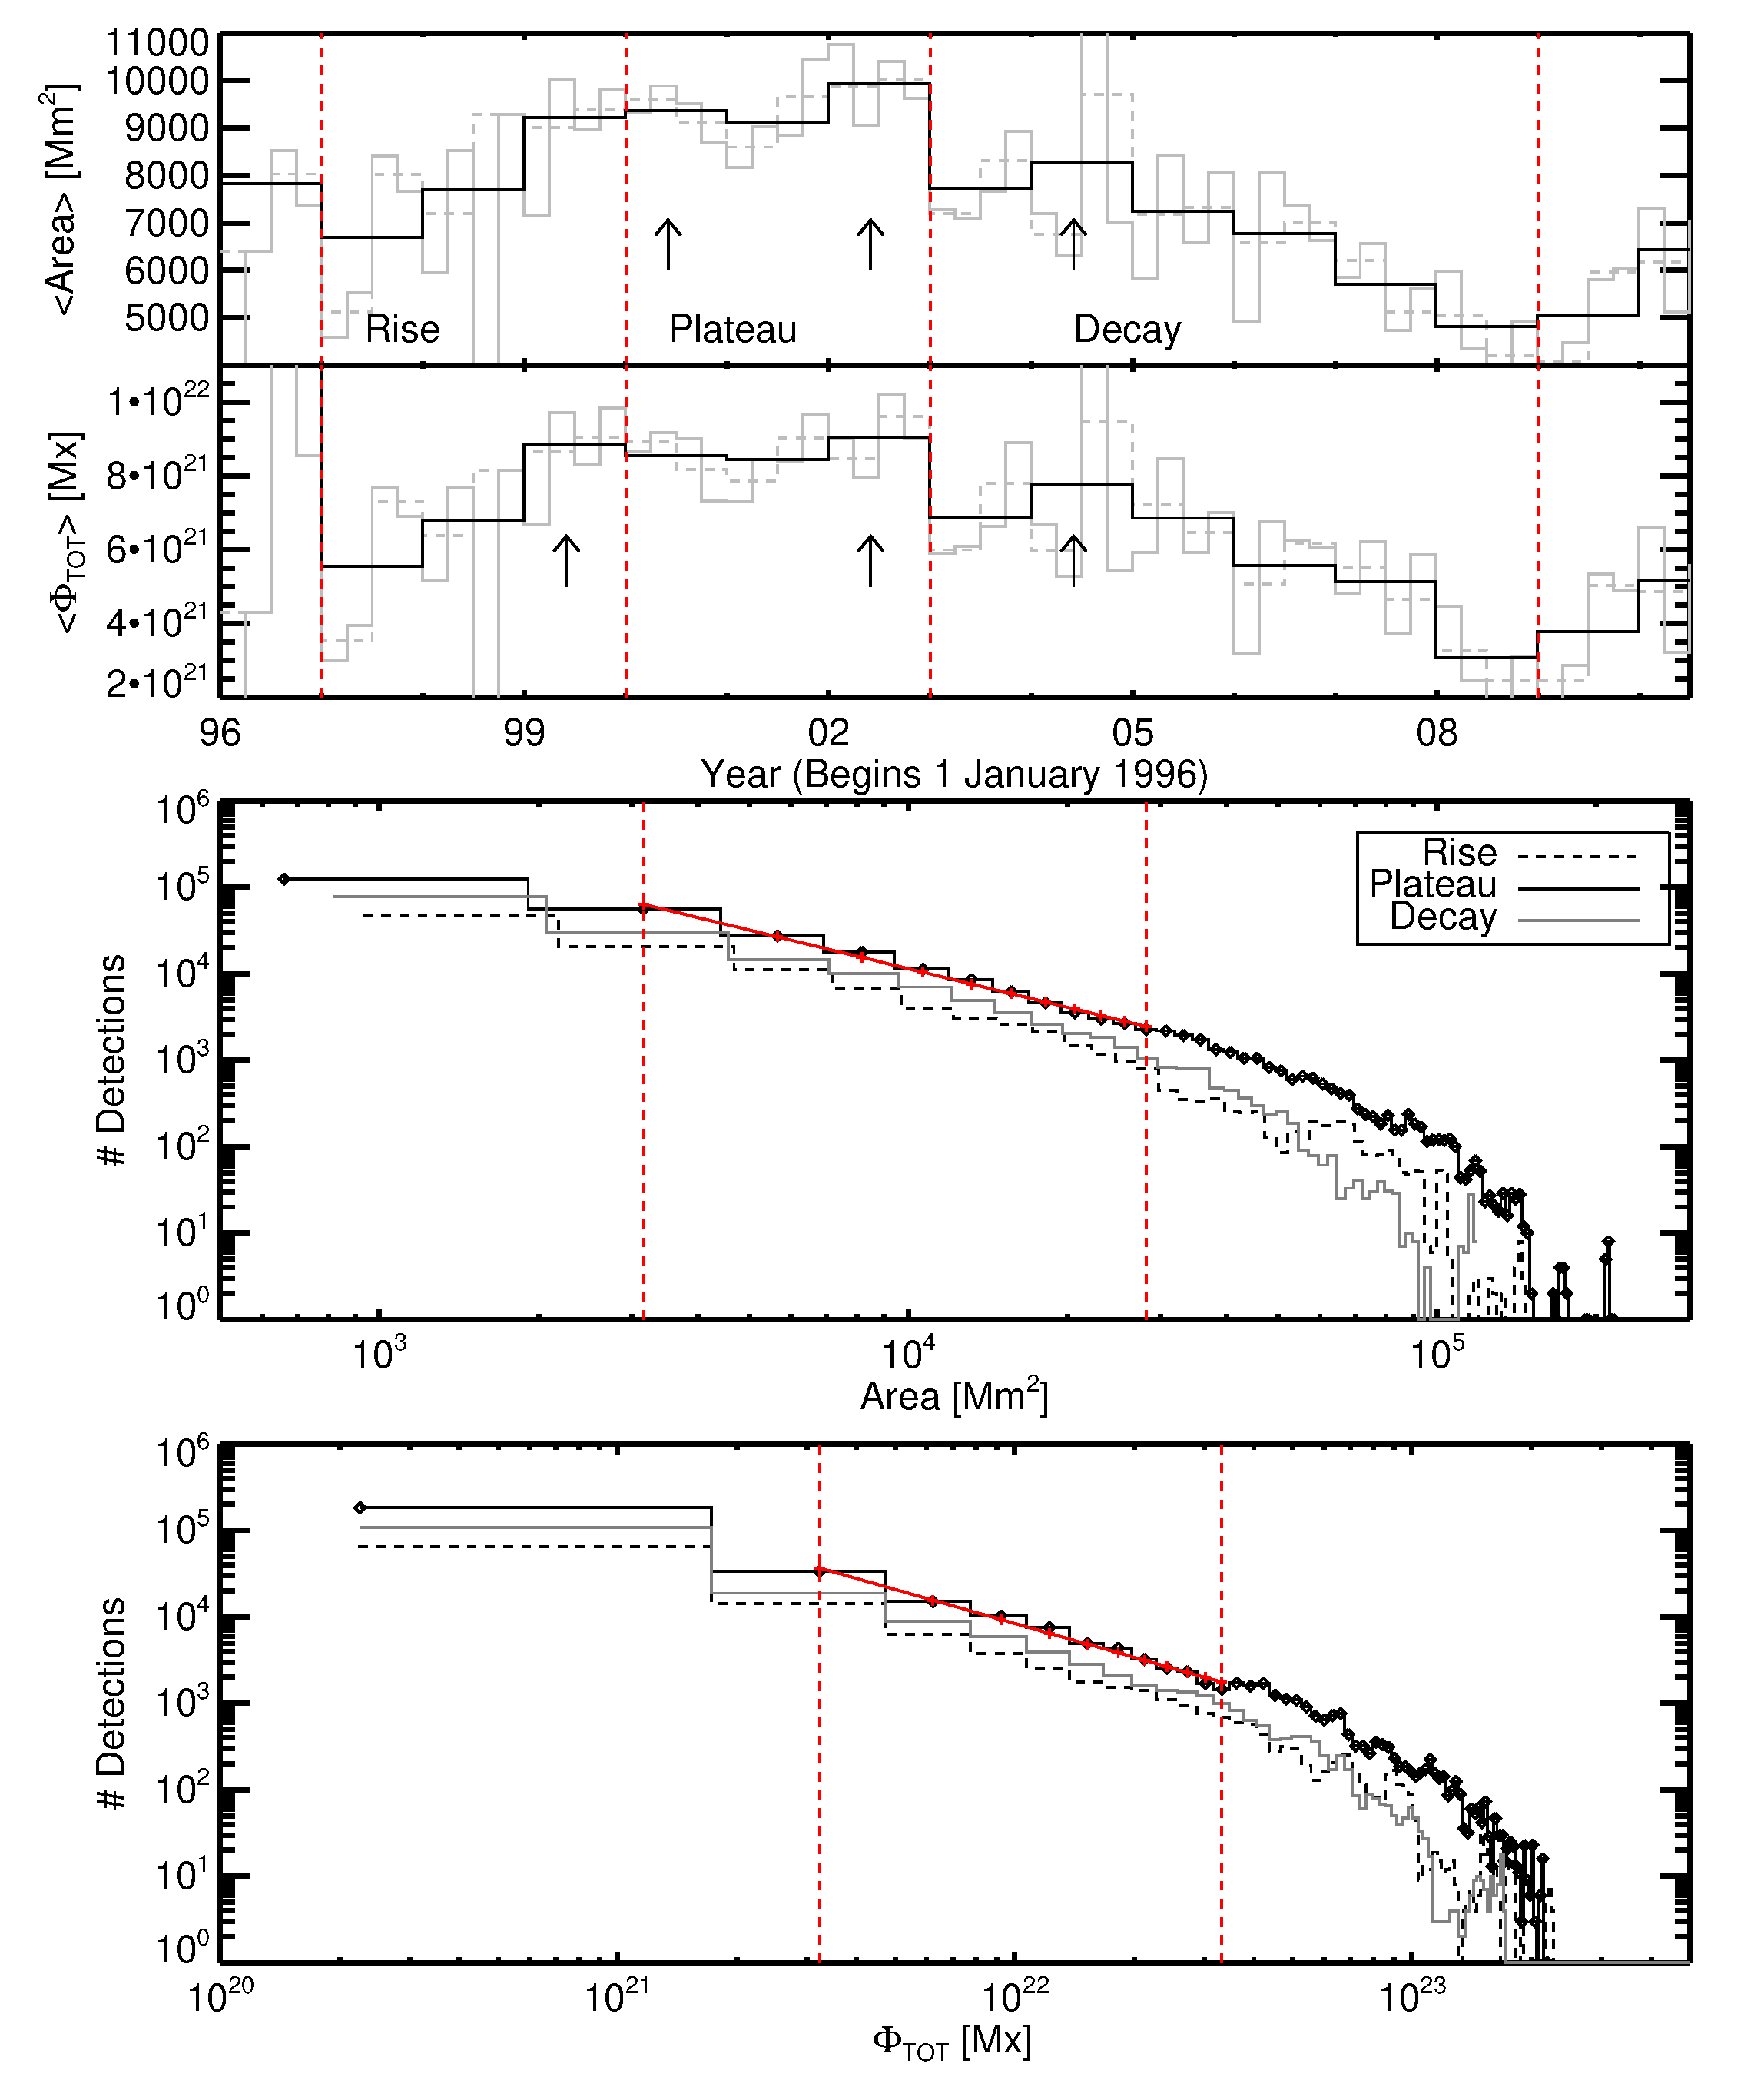
\includegraphics[width=0.9\textwidth,angle=0]{plot_2_phase_cycle_ar_prop.eps}}
\caption[The distribution of AR area and flux over the solar cycle.]{\emph{Top}: Average magnetic feature area and $\Phi_{\mathrm{tot}}$ in yearly bins (black line). Vertical lines denote beginning and end of solar cycle phases. Arrows indicate peaks in $\langle$area$\rangle$ and $\langle\Phi\rangle$. \emph{Middle}: Distributions of detection areas for ``rise" (dashed line), ``plateau" (black line), and ``decay" (gray line) phases defined in \emph{top} panel. A power-law fit to the rise-phase distribution is indicated by the straight red line. The vertical red dashed lines denote the range of the fit. \emph{Bottom} Same as \emph{middle} panel for $\Phi_{\mathrm{tot}}$.}
\label{plot_2_phase_cycle_ar_prop}
\end{figure}

It is clear that the latitude distribution of \glspl{AR} changes over the solar cycle, but the magnetic area (size) and $\Phi_{\mathrm{tot}}$ are also observed to change. The top panel of Figure~\ref{plot_2_phase_cycle_ar_prop} shows the mean area and $\Phi_{\mathrm{tot}}$ in yearly bins over the rise, maximum, and decay phases. Three low peaks are observed in each plot, two of which are coincident with the double peaks in total observed flux discussed earlier. A third peak is observed a year into the decay phase of the cycle, which is not as readily apparent in the previous plots. The average properties increase with the rise of the cycle, are roughly constant during the plateau, and decrease over the decay phase; this agrees with the findings of \citet{tang:1984}. Interpreting this plot alone, lower mean property values at solar minimum could either be due to an excess of small detections, or a lack of large detections relative to other times. Due to the large bins (1\,year) and the number of detections ($\sim$10$^4$), it is not likely that these peaks are merely statistical fluctuations. 

\begin{table}[!t]
\caption{Power-law fits to distributions of AR area and $\Phi_{\mathrm{tot}}$.}
\label{table_2_plaw_fits}
\centerline{\begin{tabular}{c c c c c}
\hline\hline
Cycle Phase & Area &  $ \mbox{Red. } \chi^2 $  & Flux &  $ \mbox{Red. } \chi^2 $  \\ 
\hline
Rise & $ -1.51 $ $ \pm $ $ 0.29 $ & $ 81.69 $ & $ -1.29 $ $ \pm $ $ 0.28 $ & $ 4.99 $ \\ 
Plateau & $ -1.49 $ $ \pm $ $ 0.26 $ & $ 186.94 $ & $ -1.30 $ $ \pm $ $ 0.25 $ & $ 83.14 $ \\ 
Decay & $ -1.50 $ $ \pm $ $ 0.28 $ & $ 168.49 $ & $ -1.27 $ $ \pm $ $ 0.27 $ & $ 27.09 $ \\ 
\hline
\end{tabular}}
\end{table}

In order to determine which is true, we plot the \gls{AR} property distributions for each phase (middle and bottom panel of Figure~\ref{plot_2_phase_cycle_ar_prop}). The area and $\Phi_{\mathrm{tot}}$ distributions are roughly power-law from $2\times10^{3}$ and $2\times10^{21}$ to $3\times10^{4}$\,Mm$^{2}$ and $3.5\times10^{22}$\,Mx, respectively. The distributions have similar power-law exponents over this range, as shown by the fits (Table~\ref{table_2_plaw_fits}). The first bin in each distribution is excluded from the fits due to the area threshold imposed by the detection method, which falls within this bin. This explains why the lowest bin falls below the power-law fits. 

Recent statistical studies of the properties of active regions have found power-law distributions for area and flux. \citet{parnell:2009} find a power-law with slope $-1.85$ for the distribution of \gls{AR} flux between $2\times10^{17}$ and $10^{23}$\,Mx. The substantial differences in the distributions between various studies are likely due in part to feature detection method \citep{deforest:2007}. Also, there are many more small features observed than large features, but feature lifetime tends to scale with size. So, many more observations of a given large feature will be included in the sample than of a given small feature. Thus, the effect of double counting the same physical feature due to the inclusion of multiple observations results in a less steep power-law slope \citep{tang:1984}. This explains why our fits ($-1.5$ for area and $-1.3$ for flux), that are based on many observations over a long period of time, are more shallow than the result of \citet{parnell:2009}, which is based on observations at single points in time. 

The distributions diverge above the power-law fit range, with the plateau phase exhibiting an excess of detections with large flux as compared with the rise and decay phases ($>$$3\times10^{22}$\,Mx). So, at solar maximum more large regions are observed than during other phases. Previous studies have found essentially the same result \citep{tang:1984,harvey:1993,meunier:2003}. This excess of large regions at the maximum of the activity cycle has also been observed in continuum sunspot observations over many cycles \citep{Hathaway:2010b}. It is possible that the excess is due to the inclusion of very large AR complexes during the plateau phase, that last much longer than any single AR. Their extended lifetime results from the continued emergence of new flux within the complex that maintains its large size.
%make this paragraph sound better!! excentuate results!


\subsection{The Global Magnetic Field}\label{subsect_imbharm}

%!!!TEMP STICK IN BUTTERFLY OF FRACTIONAL IMBALANCE TO SHOW REGIONS TOWARD EQUATOR ARE MOSTLY FLUX BALANCED

%PLOT 4. \gls{MDI} BUTTERFLY DIAGRAM
\begin{figure}[!t]
\centerline{\includegraphics[width=0.9\textwidth,angle=0]{plot_4_magbutt_arsignflux.eps}}
\caption[Magnetic butterfly diagram of mean signed field.]{\emph{Top}: Magnetic butterfly diagram ($1^{\circ}$ latitude and 27\,day time binning) of mean signed magnetic field. \emph{Bottom}: Total magnetic feature $\Phi_{\mathrm{net}}$ with binning the same as the \emph{top} panel.}
\label{plot_4_magbutt_arsignflux}
\end{figure}

The top panel of Figure~\ref{plot_4_magbutt_arsignflux} shows the mean magnetic field for each latitude over the solar cycle. This image allows us to draw several conclusions. In the northern hemisphere, the polar field begins as positive and reverses to negative around January\,2000. Large unipolar regions of negative flux can be seen to progress poleward, leading to the reversal. At about the same time an excess of positive flux is observed in the low-latitude active region belt.  The same is observed in the southern hemisphere, but with reversed polarities. Similar large-scale unipolar regions are not observed to move toward the equator during 1997\,--\,2000 (when they would be visible). So, It is reasoned that the low latitude flux imbalance is primarily a result of one polarity of magnetic flux being preferentially dragged poleward due to the combination of meridional flow and Joy's law, as is the accepted view \citep[see][and references therein]{Sheeley:2005}. This phenomena is described in Section\,\ref{section:sscycle}.

The SMART detections of individual ARs are binned in time and latitude, resulting in the image shown in the bottom panel of Figure~\ref{plot_4_magbutt_arsignflux}. The same polarity imbalances are observed in each hemisphere as in the top panel (albeit, less clearly); excess positive at low latitudes in the north and negative in the south. Since \glspl{AR} are east-west oriented, it might be assumed that the observed polarity imbalances in the active region belt are created due to features being partially out of the $60^{\circ}$ field of view. To rule out this possibility, $\Phi_{\mathrm{net}}$ is determined for detected features with boundaries completely within $\pm60^{\circ}$ longitude. Alternatively, if there was a net East-West tilt in fields from the normal to the surface of a flux balanced AR, one polarity would appear stronger in the western hemisphere while the other would appear stronger in the eastern hemisphere. This effect would be averaged out in our case, since the data are binned by 27\,days.

A flux balanced magnetic feature can have completely closed magnetic fields. However, a feature which has an excess flux of one polarity must have field which is either quasi-open (connected to the solar wind) or connected to excess flux of the opposite polarity some distance away on the solar surface. In the case of the observed excess flux in Figure~\ref{plot_4_magbutt_arsignflux} the low latitude excess flux (which is summed over longitude) is likely connected trans-equatorially, and to the high latitude excess \citep{Choudhary:2002}. The high latitude excess flux is likely connected to the poles.


%PLOT 5. FLUX IMBALANCES
\begin{figure}[!t]
\centerline{\includegraphics[width=0.9\textwidth,angle=0]{plot_5_5_fluximbal_hi_lo.eps}}
\caption[The $\Phi_{\mathrm{net}}$ measured in each hemisphere.]{\emph{Top}: Total $\Phi_{\mathrm{net}}$ determined from $\langle B_{\mathrm{signed}}\rangle$ in the magnetic butterfly diagram (poleward of detected features; $\Phi_{\langle B \rangle,HI}$) in northern (red) and southern (blue) hemispheres. \emph{Bottom}: Summed $\Phi_{\mathrm{net}}$ in the active longitudes detected in magnetic features (thick solid lines). 
%and using the magnetic butterfly diagram (dashed lines; $\Phi_{\langle B \rangle,LOW}$). 
The subscript $HI$ denotes the latitude range from the $\Phi$-edge shown in the top panel of Figure\,\ref{plot_1_analyze_fluxbflydiag} up to $\pm$54$^\circ$, while $LOW$ denotes the range from the $\Phi$-edge down to the equator.}
\label{plot_5_fluximbal_hi_lo}
\end{figure}

To determine the total imbalanced flux in detected \glspl{AR} at low latitudes, we sum their $\Phi_{\mathrm{net}}$ in each hemisphere using the data shown in the bottom panel of Figure~\ref{plot_4_magbutt_arsignflux}. 
Flux imbalances in the top panel of Figure~\ref{plot_4_magbutt_arsignflux} are quantified by defining two zones in each hemisphere using the poleward edges of the $\Phi_{\mathrm{tot}}$$>$$0$ detection mask shown in the top panel of Figure~\ref{plot_1_analyze_fluxbflydiag}: the high-latitude region is defined to be between the poleward edge of the detection mask and $54^{\circ}$ (top panel of Figure~\ref{plot_5_fluximbal_hi_lo}); the low-latitude region is defined to be between the equatorward and poleward edges of the detection mask (bottom panel of Figure~\ref{plot_5_fluximbal_hi_lo}). 

The upper bound for high-latitude flux ($\theta_{\mathrm{max}}$) is determined by estimating the distance that flux from low-latitude magnetic features is carried poleward by the meridional flow during the time interval of the $\sim$6\,month activity bursts mentioned in discussion of Figure~\ref{plot_0_cycletseries_vs_fluxbflydiag}. This is calculated by,
\begin{equation}
\Delta \theta = v_{\mathrm{flow}}\Delta t \times \frac{360^{\circ}}{2\pi R_{\odot}} \mbox{\,,}
\end{equation}
where $\theta$ is heliographic latitude, $\Delta t$ is chosen to be 6\,months, $v_{\mathrm{flow}}$ is a characteristic meridional flow speed (chosen to be 15\,m\,s$^{-1}$ from measurements in \citet{Hathaway:2010}), and $R_{\odot}$ is the solar radius. Assuming most of the \glspl{AR} emerge below 35$^{\circ}$, we add $\Delta \theta$, and calculate a $\theta_{\mathrm{max}}$ of 54$^\circ$. 
Using this value for $\theta_{\mathrm{max}}$, high-latitude flux measurements should include the majority of the poleward moving flux from a given activity burst.
%we reason the phase lag between \gls{AR} and QS flux measured in zharkov 2008 is for this reason

To calculate the total net flux at a given latitude we take the mean magnetic field measured in each latitude band (from the magnetic butterfly diagram in the bottom panel of Figure~\ref{plot_4_magbutt_arsignflux}) and multiply by the area covered by a band encircling all longitudes. This yields the net flux in a given latitude range ($\Delta \theta=\theta_2-\theta_1$) on the Sun at a given time,
\begin{equation}
\Phi_{\langle B \rangle}=\langle B \rangle 2\pi R_{\odot}^2 (\sin\theta_2 - \sin\theta_1 ) \mbox{\,,}
\end{equation}
where $\langle B \rangle$ is the averaged signed magnetic field. These flux measurements are compared to the summed \gls{AR} $\Phi_{\mathrm{net}}$ at low latitudes, as shown in Figure\,\ref{plot_5_fluximbal_hi_lo}.

We find both the low- and high-latitude imbalances to be of opposite polarity in each hemisphere. Additionally, for each hemisphere, polarity imbalances are opposite for the high and low latitudes. By comparing $\Phi_{\mathrm{net}}$ (determined from \gls{SMART} detections) 
%and $\Phi_{\langle B \rangle}$ for low latitudes ($\Phi_{\langle B \rangle,LOW}$) 
with $\Phi_{\langle B \rangle}$ for high latitudes (determined from the magnetic butterfly diagram), we can see that the flux imbalance in the active latitudes is of similar magnitude for the first half of the solar cycle, but opposite in polarity to that at high latitudes. This is the first time these measurements have been directly quantitatively compared. 

Since significant (opposite) imbalances in flux are observed for each hemisphere, this implies that flux cancellation at the equator cannot be rapid enough to offset the missing flux carried to the poles by the meridional flow. It is likely that the excess flux at low latitudes (contained in the leading polarities of \glspl{AR}) was not then carried to the equator because the leading poles of \glspl{AR} decay more slowly than the trailing. The excess flux may be contained in the stronger magnetic fields of the leading poles, which, if anchored significantly below the photosphere could then resist the surface meridional flows, unlike the weaker trailing poles that were carried much more swiftly to the north and south poles. In a sense, the system is like panning for gold. The loose sand (representing weak magnetic fields) is washed away by the flow of the water, while the gold nuggets (representing stong magnetic fields) stay planted firmly in the pan.

The reason for the large difference in the magnitude of $\Phi_{\mathrm{net}}$ and $\Phi_{\langle B \rangle}$ after 2001 may be due to the lower latitudes at which sunspot groups begin emerging. The meridional flow may not be strong enough at these latitudes to preferentially carry one polarity to high latitudes, resulting in the small values of $\Phi_{\langle B \rangle}$. Also, one polarity of flux may preferentially cancel at the equator, resulting in the large values seen in $\Phi_{\mathrm{net}}$ at this time.
%The reason $\Phi_{\mathrm{net}}$ differs from $\Phi_{\langle B \rangle,LOW}$ is due the methods used to calculate them. The properties of \gls{AR} detections averaged over a rotation are used determine $\Phi_{\mathrm{net}}$, while raw magnetograms are averaged to determine $\Phi_{\langle B \rangle,LOW}$ and $\Phi_{\langle B \rangle,HI}$.

%LASCO DATA
Magnetic field-line traces are overlaid on white-light coronagraph images to compare the magnetic structure in the lower corona to that further out. This is done using extrapolations from the global \gls{PFSS} model\footnote{The model runs rely on MDI LOS data and can be downloaded and visualised using the PFSS widget available through SolarSoft, as was done in this work. Documentation for the PFSS code is available here: \url{http://www.lmsal.com/\~derosa/pfsspack/}} described in \citet{Schrijver:2003} and Level 1 \emph{SoHO}/Large Angle and Spectrometric Coronagraph Experiment \citep[LASCO;][]{brueckner:1995} data, as shown in Figure~\ref{plot_3_lasco_pfss}. The coronagraph images are radially filtered by dividing out the average intensity in 5 pixel-width annuli. The coronagraph data and \gls{PFSS} extrapolations are matched as close as possible in time. 

These images show regions of enhanced density in the extended corona. The shape of these regions is determined by large-scale magnetic fields. We observe the majority of imaged helmet streamers to have roughly the same configuration as the dominant modeled closed-loop structures. The configuration of surface magnetic features is expected to match the global configuration of the atmosphere exterior to the Sun \citep{Schrijver:2003}. \citet{Wang:2009} compare modeled coronal emission (determined using a \gls{PFSS} algorithm) to LASCO data, remapped to time-latitude space, finding good agreement. 

%PLOT 3. \gls{PFSS} VS. LASCO
\begin{landscape}
\begin{figure}[!t]
\centerline{\includegraphics[width=1.5\textwidth,angle=0,clip=true]{plot_3_lasco_pfss_2_ill10.eps}}
\caption[Comparison between PFSS extrapolations and white-light images.]{Comparison between global PFSS extrapolations and white-light coronagraph observations. Color denotes closed (black), positive open (light-gray) and negative open (dark-gray) field lines.}\label{plot_3_lasco_pfss}
\end{figure}
\end{landscape}

Differences occur because the structure of the corona is dynamic on the scale of hours, while photospheric features, once emerged tend exhibit dynamics on the scale of days. For instance, transient phenomena (coronal mass ejections and out-flows) may occur, which do not cause significant structural changes in the photosphere. Differences between the extrapolated magnetic structures and enhanced coronal density configuration may be caused by this as well as by the methods used to generate a 360$^\circ$ map of the solar surface, utilised by the \gls{PFSS} model. 

Rapid flux emergence could occur in the photosphere that is beyond the assimilation edge of the \gls{PFSS} model. The model used in this work relies on photospheric field maps produced by assimilating new flux at the east edge of the solar disk as it rotates into view. Any flux beyond that edge is estimated from that which has rotated off the west edge of the disk $\sim$two weeks before. Regions which have emerged on the backside of the Sun and not yet rotated on disk will therefore not be included in a given extrapolation. Because reliable magnetic field observations of the far side of the Sun are not available and the dynamic timescale of the solar surface and atmosphere is much shorter than the rotation period, any \gls{PFSS} results can not be a true snap shot of the Sun, and must smear out measurements in time and space. Finally, \gls{LOS} effects in the magnetograms, as discussed in Chapter~\ref{chapter:method_SMART}, such as false \glspl{PSL}, can also affect the field extrapolation.

%PLOT -. SPHERICAL HARMONIC MODE EXAMPLES
\begin{figure}[!t]
\centerline{\includegraphics[width=0.9\textwidth,angle=0]{plot_6_5_spheric_harm_examp2.eps}}
\caption[Spherical harmonic visualisations.]{Examples of axially symmetric and hemispherically antisymmetric spherical harmonics. White represents positive and black represents negative regions of $\Psi(r,\theta,\phi)$ at radius $R_{\odot}$. Sections of the $\langle B_{\mathrm{signed}} \rangle$ butterfly diagram are included adjacent to each mode for context.}
\label{plot_6_5_spheric_harm_examp}
\end{figure}

These magnetic field extrapolations are used to determine how the global magnetic field changes over the solar cycle. Spherical harmonics, as defined by Equation \ref{eqn_harm_coeff}, are used here to describe the large-scale field topology. At different phases of the solar cycle the field can be described by different modes. When there are no magnetic features detected, such as during solar minimum, the global field configuration is that of a dipole $(\ell=1,m=0)$, as shown in the first panel of Figure~\ref{plot_6_5_spheric_harm_examp}. After the first active regions of the cycle have emerged and begun to decay, 3 regions of opposite polarity are visible at different latitudes, so the global field gains a significant $(\ell=5,m=0)$ moment (third panel). Finally, after the north and south poles have switched polarity, the following polarity of an active region is the same as that of its nearest pole, and there is a significant $(\ell=3,m=0)$ moment in the solar field (second panel). 

Near the solar surface, these harmonic modes are not as useful for describing the magnetic field structure because of the presence of localised strong-field features (i.e., plage and sunspots). But, a few $R_\odot$ from the surface low-order modes begin to dominate. This is because the magnetic field strength falls off faster with the higher-order modes.


%PLOT 6. POLAR FIELDS AND MULTI-POLAR COEFFICIENTS
\begin{figure}[!t]
\centerline{\includegraphics[width=0.9\textwidth,angle=0]{plot_6_polarb_sphereharm.eps}}
\caption[Global magnetic field spherical harmonic strengths over time.]{\emph{Top}: Polar field strengths in the northern (Red) and southern (Blue) hemispheres, determined from the $\langle B \rangle$ map (top panel of Figure\,\ref{plot_4_magbutt_arsignflux}). Dashed lines indicate field values sampled from higher latitudes than the those indicated by the solid line.  \emph{Bottom}: Spherical harmonic coefficients for three different modes.}
\label{plot_6_polarb_sphereharm}
\end{figure}

The top panel of Figure~\ref{plot_6_polarb_sphereharm} shows the polar field strengths averaged over two latitude bands. The southern hemisphere field appears to reverse before the northern one. Field reversal occurs smoothly over 2\,--\,3\,years in the northern hemisphere while it happens in several $\sim$year timescale bursts in the south. This is similar to the progression of southern $\Phi_{\mathrm{tot}}$ (Figure~\ref{plot_0_cycletseries_vs_fluxbflydiag}), which exhibits large peaks and troughs.

To determine how significant each of the harmonic modes are to the global field configuration, we can compare the harmonic coefficients of each mode (see Equation \ref{eqn_harm_coeff}) over time, as calculated by the \gls{PFSS} model. At solar minimum, when the field strengths are largest and the fewest magnetic features are present, the dipole $(\ell=1,m=0)$ harmonic coefficient is largest (black line in bottom panel). There is also a significant $(\ell=3,m=0)$ moment during this time, which is probably due to the presence of a single bipolar magnetic feature on disk. As more active regions emerge and decay, the $(\ell=5,m=0)$ mode becomes dominant from around 1999 to 2001. From 2001 to mid 2004, the $(\ell=3,m=0)$ mode is dominant since the poles have switched polarity. When few enough \glspl{AR} are present, the dipolar mode becomes dominant again, from mid 2004 onward.


\section{Conclusions and Future Work}\label{discussion}

%SUMMARY OF RESULTS, WHATS NEW?
In this chapter, we use automated magnetic feature extraction to determine the properties of a large sample of magnetic features that emerge into the solar photosphere. The evolution of large-scale magnetic fields can be characterised by studying the dynamic properties of \gls{AR} emergence. We support some previous work on the magnetic solar cycle, as well as provide some new insights and draw some new conclusions. A summary of our results is as follows: 
\begin{itemize}
\item The double peak observed in the solar activity cycle only occurs in the southern hemisphere and activity in the northern hemisphere exhibits a much smoother rise and decline over the cycle. This indicates that the subsurface production of strong magnetic field structures due to the magnetic dynamo is asymmetric. 
\item The emergence of features of largest magnetic flux are most confined in latitude and this latitude moves equatorward over the solar cycle. This could indicate the magnetic flux distribution at the base of the tachocline at the start of the solar cycle. Alternatively, this could be related to the equatorward progression of the torsional oscillation, which may be responsible for the onset of \gls{AR} emergence at a given latitude at the start of a solar cycle. 
\item There is an excess of magnetic features with large flux in the plateau phase of the solar cycle. This could result from the formation of sunspot nests or active longitudes, in which multiple magnetic features emerge at the same position on the solar surface\footnote{See the analysis of NOAA 10365 in Chapter~\ref{chapter:results_activity}.}, sometimes forming large \gls{AR} complexes.
\item The flux imbalance in the north (south) active latitudes is positive (negative) in polarity and of the same order of magnitude to that at north (south) high latitudes for cycle 23. This is the first time this comparison has been made. We suggest that the observed flux imbalance results from one polarity of magnetic flux being preferentially carried to high latitudes by the meridional flow.
\item The dominance of certain global magnetic field spherical harmonic moments over the solar cycle is a result of the large-scale distribution of imbalanced flux. Alternating latitudinal bands of imbalanced flux which vary over the solar cycle are shown to have a significant impact on the global magnetic field.
\end{itemize}

%AGREE/DISAGREE WITH PREVIOUS WORK
Many authors, including \citet{Temmer:2006}, have shown that the emergence of sunspot groups is hemispherically asymmetric. This work presents one of the few comparisons of hemispheric flux imbalance. \citet{meunier:2003} compares the flux distribution of magnetic features in each hemisphere, finding different excesses of detected features in each hemisphere depending on the threshold used in their detection method, while our results show a clear dominance of each hemisphere at different times during the solar cycle.

%ISSUES WITH OUR METHODS ETC
The use of \gls{SMART} for detecting \glspl{AR} affects the measurement of flux imbalance. Weaker fields at the edges of trailing plage regions associated with \glspl{AR} are less likely to be included in the \gls{SMART} detection contours than the dense fields of sunspots. Thus, if a region emerges flux balanced, it will be left with an excess of dense leading-polarity flux as the trailing polarity decays. However, the same dominant-polarity pattern is observed in the butterfly diagram of flux imbalance (Figure~\ref{plot_4_magbutt_arsignflux}) constructed using raw magnetograms (top panel) and the one constructed using \gls{SMART} detections (bottom panel). Thus, it is likely that the observed polarity excesses are merely exaggerated, rather than incorrect.  

%PHYSICAL IMPLICATIONS
%FUTURE WORK

This work has resulted in the characterisation of magnetic features and their emergence over the solar cycle. Although the choice of divisions for solar cycle phases differs, our results essentially agree with those of \cite{meunier:2003} in that there is an excess of large features around solar cycle maximum. This is important for constraining dynamo models. For instance, we have determined the latitudinal distribution of the flux and size of detected features over time and these results can be tied to a model of buoyant flux rope deflection due to the coriolis force to constrain their subsurface properties. A future detailed comparison of sunspot group detections to the residual meridional flow and differential rotation (torsional oscillation) could indicate the nature of their relationship. Currently, it is only clear that magnetic activity and the torsional oscillation is  well correlated in time and latitude \citep{Hathaway:2011}. The next step in studying the solar activity cycle is to tie observations of emergent solar features to both phenomenological and mean-field dynamo models of the solar convection zone. 



% ---------------------------------------------------------------------------
%: ----------------------- end of thesis sub-document ------------------------
% ---------------------------------------------------------------------------

